\section{Background}
\label{sec:background}
%Use only \lambda type KRR regression, rather than GP and posterior mean and \sigma^; We need to 统一表达方式

\subsection{Kernel ridge regression}
Let \(\{(x_i,y_i)\}_{i=1}^N\) be training data, with
\(x_i\in\mathbb R^d\) and \(y_i\in\mathbb R\). For a positive-definite
kernel \(k\) with reproducing kernel Hilbert space (RKHS) \(\mathcal H\),
KRR solves
% only H not H_k
\[
    \hat f
    = \argmin_{f\in\mathcal H}
    \sum_{i=1}^N \bigl(f(x_i)-y_i\bigr)^2
    +
    \lambda \|f\|_{\mathcal H}^2.
\]
We use the unnormalized KRR convention: the data-fit term is not divided by
\(N\). Thus a fixed \(\lambda\), such as \(\lambda=0.1\), remains a fixed
diagonal regularization level as \(N\) changes, while its strength relative to
the \(O(N)\) unregularized Fourier system decreases. Under the averaged-loss
convention, the equivalent coefficient would be \(\lambda/N\).
The representer theorem gives
% exist some alpha
\(\hat f(x)=\sum_{i=1}^N\alpha_i k(x,x_i)\). With
\(\K_{ij}=k(x_i,x_j)\), \(\y=(y_1,\ldots,y_N)^\top\), and
\(\alphavec=(\alpha_1,\ldots,\alpha_N)^\top\), the coefficients satisfy
\((\K+\lambda\I_N)\alphavec=\y\). This is an \(N\times N\) dense system
\cite{aronszajn1950theory,kimeldorf1971some,scholkopf2001generalized,rasmussen2006gaussian}.
%Computation Memory Cost; direct inverse and iterative solvers
% later to Fourier
\subsection{Weight-space KRR}
Suppose the kernel is approximated by \(M\) features:
\[
    k(x,x')
    \approx
    \widetilde k(x,x')
    =
    \sum_{j=1}^M \phi_j(x)\overline{\phi_j(x')},
    \qquad \phi_j:\mathbb R^d\to\mathbb C .
\]
Let \(\Phimat_{ij}=\phi_j(x_i)\), so
\(\widetilde{\K}=\Phimat\Phimat^*\). For this fixed approximate kernel, the
equivalent \(M\times M\) system is
\[
    (\Phimat^*\Phimat+\lambda \I_M)\betavec=\Phimat^*\y, \quad
    \betavec=(\beta_1,\ldots,\beta_M)^\top\in\mathbb C^M.
\]
The corresponding coefficients obey \(\betavec=\Phimat^*\alphavec\) and
\(\alphavec=(\y-\Phimat\betavec)/\lambda\); these relations follow directly
from the data-space and weight-space systems
\cite{rasmussen2006gaussian,greengard2025efgp,barnett2024uniform}.
% too much concept
% mix the idea
%
\subsection{Equispaced Fourier expansion}
\label{subsec:equispaced-fourier-expansion}
\paragraph{Kernel approximation}
\label{subsec:fourier-expansion}

We consider translation-invariant kernels with \(d\leq3\) in the experiments.
By Bochner's theorem, such a kernel has a nonnegative spectral density
\(\widehat k\) such that
\[
k(x,z)
=
\int_{\mathbb R^d}
\widehat k(\omega)
 e^{2\pi i\langle \omega,x-z\rangle}\,d\omega .
\]
We approximate this integral on the grid
\(J_m=\{-m,-m+1,\ldots,m\}^d\), which contains
\(M=(2m+1)^d\) frequencies. The resulting finite sum is
\cite{bochner1933monotone,greengard2025efgp,barnett2024uniform}
\[
\widetilde k(x,z)
=
\sum_{j\in J_m}
 h^d\widehat k(hj)
 e^{2\pi i h\langle j,x-z\rangle}.
\]
The design matrix \(\Phimat\in\mathbb C^{N\times M}\) is
\[
  \Phimat_{n,j}=\phi_j(x_n),\quad \phi_j(x)
=
\sqrt{h^d\widehat k(hj)}
 e^{2\pi i h\langle j,x\rangle},
\qquad j\in J_m .
\]
For the kernels studied here, the approximation can reach high accuracy with
\(M\ll N\) \cite{greengard2025efgp,barnett2024uniform}.



\paragraph{Fast matrix-vector products}
%Define D,F, g=F^*F, H=\Phimat^*Phi, A= H+\lambda I_M
%Show that D is diagonal and G is Toeplitz, then convolution with fast NUFFT of v to Gv , then v to Av
Write \(\Phimat=FD\), where
\[
\begin{aligned}
F_{n,j}&=e^{2\pi i h\langle j,x_n\rangle},
&F&\in\mathbb C^{N\times M},\\
D_{j,\ell}&=\sqrt{h^d\widehat k(hj)}\,\delta_{j\ell},
&D&\in\mathbb R^{M\times M},
\qquad j,\ell\in J_m.
\end{aligned}
\]
Because \(D\) is real and diagonal, the Fourier weight-space system is
\begin{equation}
    A\betavec=b,
    \qquad A=DGD+\lambda\I_M,
    \qquad G=F^*F,
    \qquad b=DF^*\y.
    \label{eq:fourier-system}
\end{equation}
Once \(h\) and \(m\) are fixed, this is the finite-dimensional system studied
below. The preconditioner changes neither \(A\), \(b\), nor its exact
solution. This does not identify the Fourier approximation with the original
KRR problem.
% show the fast computation method，尽量精简 
Because \(G_{j,\ell}=g_{\ell-j}\), \(G\) is a
\(d\)-level Toeplitz matrix determined by
\[
    g_r
    =
    \sum_{n=1}^N
    e^{2\pi i h\langle r,x_n\rangle},
    \qquad r\in J_{2m}.
\]
The generator costs \(O(N+M\log M)\) to compute with a type-1 NUFFT.
Thereafter, padded FFTs apply \(G\) as a nonperiodic convolution in
\(O(M\log M)\) time
\cite{greengard2025efgp,barnett2019finufft,shih2021cufinufft}. The same
type-1 NUFFT computes the right-hand side in \cref{eq:fourier-system}, since
\((F^*\y)_j=\sum_{n=1}^N
e^{-2\pi i h\langle j,x_n\rangle}y_n\). Thus setup costs
\(O(N+M\log M)\), and the product
\(Au=D\,G(Du)+\lambda u\) costs \(O(M\log M)\), independently of \(N\).
With \(t_{\rm iter}\) iterations, the complete solve costs
\(O(N+M\log M+t_{\rm iter}M\log M)\)
\cite{greengard2025efgp,barnett2024uniform}.



\subsection{Preconditioned conjugate gradient}
\label{subsec:pcg}
% citation: the speed of CG
% citation: when PCG could accelerate
% \epsilon define here, relative error defind; iterative method, and the number of iteration, more precisely --- statement:....., then run .... to reach.
Since \(A\) is Hermitian positive definite, CG solves \(A\betavec=b\) using
only products with \(A\). Its standard worst-case bound requires
\(O(\sqrt{\kappa(A)}\log(1/\varepsilon))\) iterations to reduce the relative
\(A\)-norm error below \(\varepsilon\)
\cite{hestenes1952methods,saad2003iterative,trefethen1997numerical}.
% highlight the kappa, the imortance the conditioning.. common idea for improving the conditiong number
% idea of preconditioning:
% matvec later: first number of iteration, then each matvec;
% on top of ...


% short but no ambiguity (no meaningless definition)
% clustering but linear the idea;
Let \(P\) be a positive-definite approximate inverse. Preconditioned CG depends
on both \(\kappa(P^{1/2}AP^{1/2})\) and the cost of constructing and applying
\(P\). The iteration is given in
\cref{app:algorithms-implementation}.


%In the EFGP system, these products are fast, but the number of iterations may still be large when \(A\) is ill-conditioned.



% In this paper, a positive definite \(P\) denotes the preconditioner application, so that PCG applies \(z_t=P r_t\). Fourier Expansion provides fast computation of matvecs. And preconditioning reduces \(n_{\mathrm{iter}}\) \cite{hestenes1952methods,saad2003iterative,trefethen1997numerical}.
% to appendix

% For CG, \(P=\I\). Its convergence depends on the condition number
% \(
%     \kappa(A)=\frac{\lambda_{\max}(A)}{\lambda_{\min}(A)} .
% \)
% More precisely, if \(\betavec_\star\) is the exact solution, then
% \begin{equation}
%     \frac{\|\betavec_t-\betavec_\star\|_A}{\|\betavec_0-\betavec_\star\|_A}
%     \leq
%     2\left(
%     \frac{\sqrt{\kappa(A)}-1}{\sqrt{\kappa(A)}+1}
%     \right)^t .
%     \label{eq:cg-rate}
% \end{equation}
% PCG replaces this dependence by the condition number of the symmetrically preconditioned matrix,
% \[
%     \kappa_P
%     =
%     \kappa(P^{1/2}AP^{1/2}).
% \] Therefore, an effective preconditioner must balance three requirements: it should substantially reduce the effective condition number \(\kappa_P\), have a low construction cost, and allow each application \(v\mapsto Pv\) to be efficiently computed.\cite{saad2003iterative,trefethen1997numerical}


% The second requirement is also satisfied. Krylov eigensolvers, such as ARPACK/eigsh\cite{ma2017eigenpro,ma2019eigenpro,lanczos1950iteration,lehoucq1998arpack}, provide efficient estimation of the top eigenvalues and eigenvectors using only$v \to Av$, while EFGP provides quick matvec computation. In addition, $v \to Pv$ is also efficient for the low rank structure of $P$.


% \begin{remark}[Computational limitation]
% For severely ill-conditioned systems with large \(M\), an effective preconditioner may require a relatively large rank \(q\). Estimating the corresponding leading eigenspace then entails many \(v \mapsto Av\). Moreover, when \(U_q\) is stored explicitly, each application of the preconditioner costs \(O(Mq)\). Consequently, the reduction in iterations may be partially offset by the computational cost of constructing and applying \(P_q\).

% \end{remark}

% For matrix A with
% \[
%     A u_i=\theta_i u_i,\qquad
%     \theta_1\geq\theta_2\geq\cdots\geq\theta_M>0,
% \]
% and let \(U_q=(u_1,\ldots,u_q)\) contain the dominant eigenvectors, with
% \[
%     \Theta_q=\diag(\theta_1,\ldots,\theta_q).
% \]
% Following the spectral-flattening idea of EigenPro
% \cite{ma2017eigenpro,ma2019eigenpro,abedsoltan2023toward}, we define
% \begin{equation}
%     P_q
%     =
%     \I_M
%     -
%     U_q\bigl(\I_q-\theta_{q+1}\Theta_q^{-1}\bigr)U_q^*,
%     \label{eq:eigenpro-type-preconditioner}
% \end{equation}
% If the eigenpairs are accurate enough, the largest \(q\) eigenvalues are
% flattened to \(\theta_{q+1}\), while the remaining eigenvalues are unchanged. Hence
% \[
%     \kappa_{P_q}(A)
%     =
%       \kappa(P_q^{1/2}AP_q^{1/2})
%       =
%     \frac{\theta_{q+1}}{\theta_M}
%     \leq
%     \frac{\theta_1}{\theta_M}
%     =
%     \kappa(A).
% \]

% \begin{remark}[Computational limitation]
% Although \(P_q\) improves the spectrum, it requires estimating the dominant eigenspace. For ill-conditioned systems with large M, this estimation may still require many matrix-vector products with \(A\). In addition, each preconditioner application costs \(O(Mq)\) when \(U_q\) is stored explicitly. Thus the benefit of reducing iterations can be partly offset by the cost of constructing and applying \(P_q\).

% \end{remark}
% This motivates a more structure-aware alternative. Instead of estimating the dominant eigenspace of \(A\) by repeated Krylov iterations, we exploit the Fourier-coordinate representation already present in EFGP. The diagonal profile of \(H=DGD\) provides a cheap proxy for the strength of each Fourier mode and leads to the active-mode score introduced below. But with only $q$ required and no other condition needed, it serves as the most versatile and robust baseline preconditioner.

% \subsection{Fourier-Mode Strength in the EFGP System}
% \label{subsec:efgp-diagonal-dominance}

% The discussion above motivates a closer look at the structure of the Equispaced Fourier approximation weight-space matrix in \eqref{eq:A-DGD} and\eqref{eq:FD}. 



% \begin{proposition}[Diagonal profile of the EFGP system]
% \label{prop:efgp-diagonal-profile}
% For \(F\), \(D\), \(G\), and \(H\) in \eqref{eq:A-DGD}--\eqref{eq:FD},
% \begin{equation}
%     |F_{n,j}|=1,
%     \qquad
%     G_{j,j}=N,
% \end{equation}
% and hence
% \begin{equation}
%     H_{j,j}
%     =
%     N |D_{j,j}|^2
%     \label{eq:H-diagonal}
% \end{equation}
% Moreover, for \(j,\ell\in J_m\),
% \begin{equation}
%     H_{j,\ell}
%     =
%     D_{j,j}D_{\ell,\ell}
%     \sum_{n=1}^N
%     e^{2\pi i h\langle \ell-j,x_n\rangle},
%     \qquad
%     |H_{j,\ell}|
%     \leq
%     N |D_{j,j}|\,|D_{\ell,\ell}|.
%     \label{eq:H-offdiag-bound}
% \end{equation}
% Equivalently,
% \begin{equation}
%     |H_{j,\ell}|
%     \leq
%     \sqrt{H_{j,j}H_{\ell,\ell}} .
%     \label{eq:H-entry-bound-diagonal}
% \end{equation}
% \end{proposition}

% This proposition shows that the strength of each Fourier coordinate is controlled by D with \(D_j= \sqrt{h^d\widehat\kappa(hj)}\). For common stationary kernels, this quantity decays at least polynomially as the frequency \(\|j\|\) grows. Therefore high-frequency coordinates have small diagonal entries in \(H\), and their interactions with other coordinates are also damped by
% \eqref{eq:H-entry-bound-diagonal}.

% \paragraph{Active Fourier Feature Sets}
% This suggests the signal-to-regularization score
% \begin{equation}
%     \rho_j
%     =
%     \frac{N |D_{j,j}|^2}{\lambda}
%     =
%     \frac{H_{j,j}}{\lambda}.
%     \label{eq:rho-score}
% \end{equation}
% Large \(\rho_j\) means that the Fourier coordinate \(j\) contributes a diagonal signal larger than the regularization scale \(\lambda\). Small \(\rho_j\) means that the coordinate is mostly dominated by the diagonal shift($\lambda I_M$) in \(A\).

% For a threshold \(\tau>0\) or a prescribed budget \(k\), define the active set
% \begin{equation}
%     S_\tau = \{j\in J_m : \rho_j > \tau\}.
%     \qquad
%     \label{eq:tau-active-set}
% \end{equation}

% Let \(j_{(1)},j_{(2)},\ldots\) be an ordering of \(J_m\) such that
% \(\rho_{j_{(1)}}\geq \rho_{j_{(2)}}\geq\cdots\). Then
% \[
%     S_k=\{j_{(1)},\ldots,j_{(k)}\}.
% \]
% where ties are broken deterministically by increasing frequency radius.

% Since \(\widehat\kappa(hj)\) is typically largest near the origin and decreases with frequency, these active sets are low-frequency sets: intervals in one dimension, disk-like sets in two
% dimensions, and ball-like sets in three dimensions. However, such sets are not generally Cartesian boxes, so the restricted matrix
% \(A_{S S}\) does not preserve the full multilevel Toeplitz structure. To retain Toeplitz structure for fast computation, we also define \(B\) as the smallest axis-aligned frequency box containing \(S\):
% \begin{equation}
%     S\subseteq B\subseteq J_m,
%     \qquad
%     B=\{-b_1,\ldots,b_1\}\times\cdots\times\{-b_d,\ldots,b_d\}.
%     \label{eq:active-box}
% \end{equation}

% Then \(G_{B B}\) is again a \(d\)-level Toeplitz matrix on a Cartesian grid, and
% \begin{equation}
%     A_{B B}
%     =
%     D_B G_{B B}D_B+\lambda \I_B
%     \label{eq:ABB-box-system}
% \end{equation}
% can be treated using the same Fourier-Toeplitz machinery as the full system.

% \paragraph{Toy data example}
% We use a two-dimensional synthetic regression problem to make the structure visible. 
% The training inputs are sampled independently as
% \[
%     x_i \sim \mathrm{Unif}([0,1]^2), \qquad i=1,\ldots,N,
% \]
% with \(N=8{,}192{,}000\). The responses are generated from
% \[
%     y_i=f(x_i)+\epsilon_i,\qquad 
%     \epsilon_i\sim\mathcal N(0,0.5^2),
% \]
% where
% \[
%     f(x_i)
%     =
%     \sin(2\pi x_{i1})
%     +0.5\cos(2\pi x_{i2})
%     +0.2\sin(2\pi(x_{i1}+x_{i2})).
% \]
% We use a Mat\'ern kernel with smoothness \(\nu=3/2\), lengthscale \(\ell=0.1\), and unit marginal variance
% \[
%     k(r)
%     =
%     \frac{2^{1-\nu}}{\Gamma(\nu)}
%     \left(\frac{\sqrt{2\nu}r}{\ell}\right)^\nu
%     K_\nu\left(\frac{\sqrt{2\nu}r}{\ell}\right),
%     \qquad \nu=\frac32,\ \ell=0.1.
% \]

% This Mat\'ern kernel is expected to be concentrated near low frequencies. Figure~\ref{fig:active-fourier-concentration} visualizes this concentration and the enclosing Cartesian active box used by our preconditioner.


% \begin{figure}[H]
% \centering
% 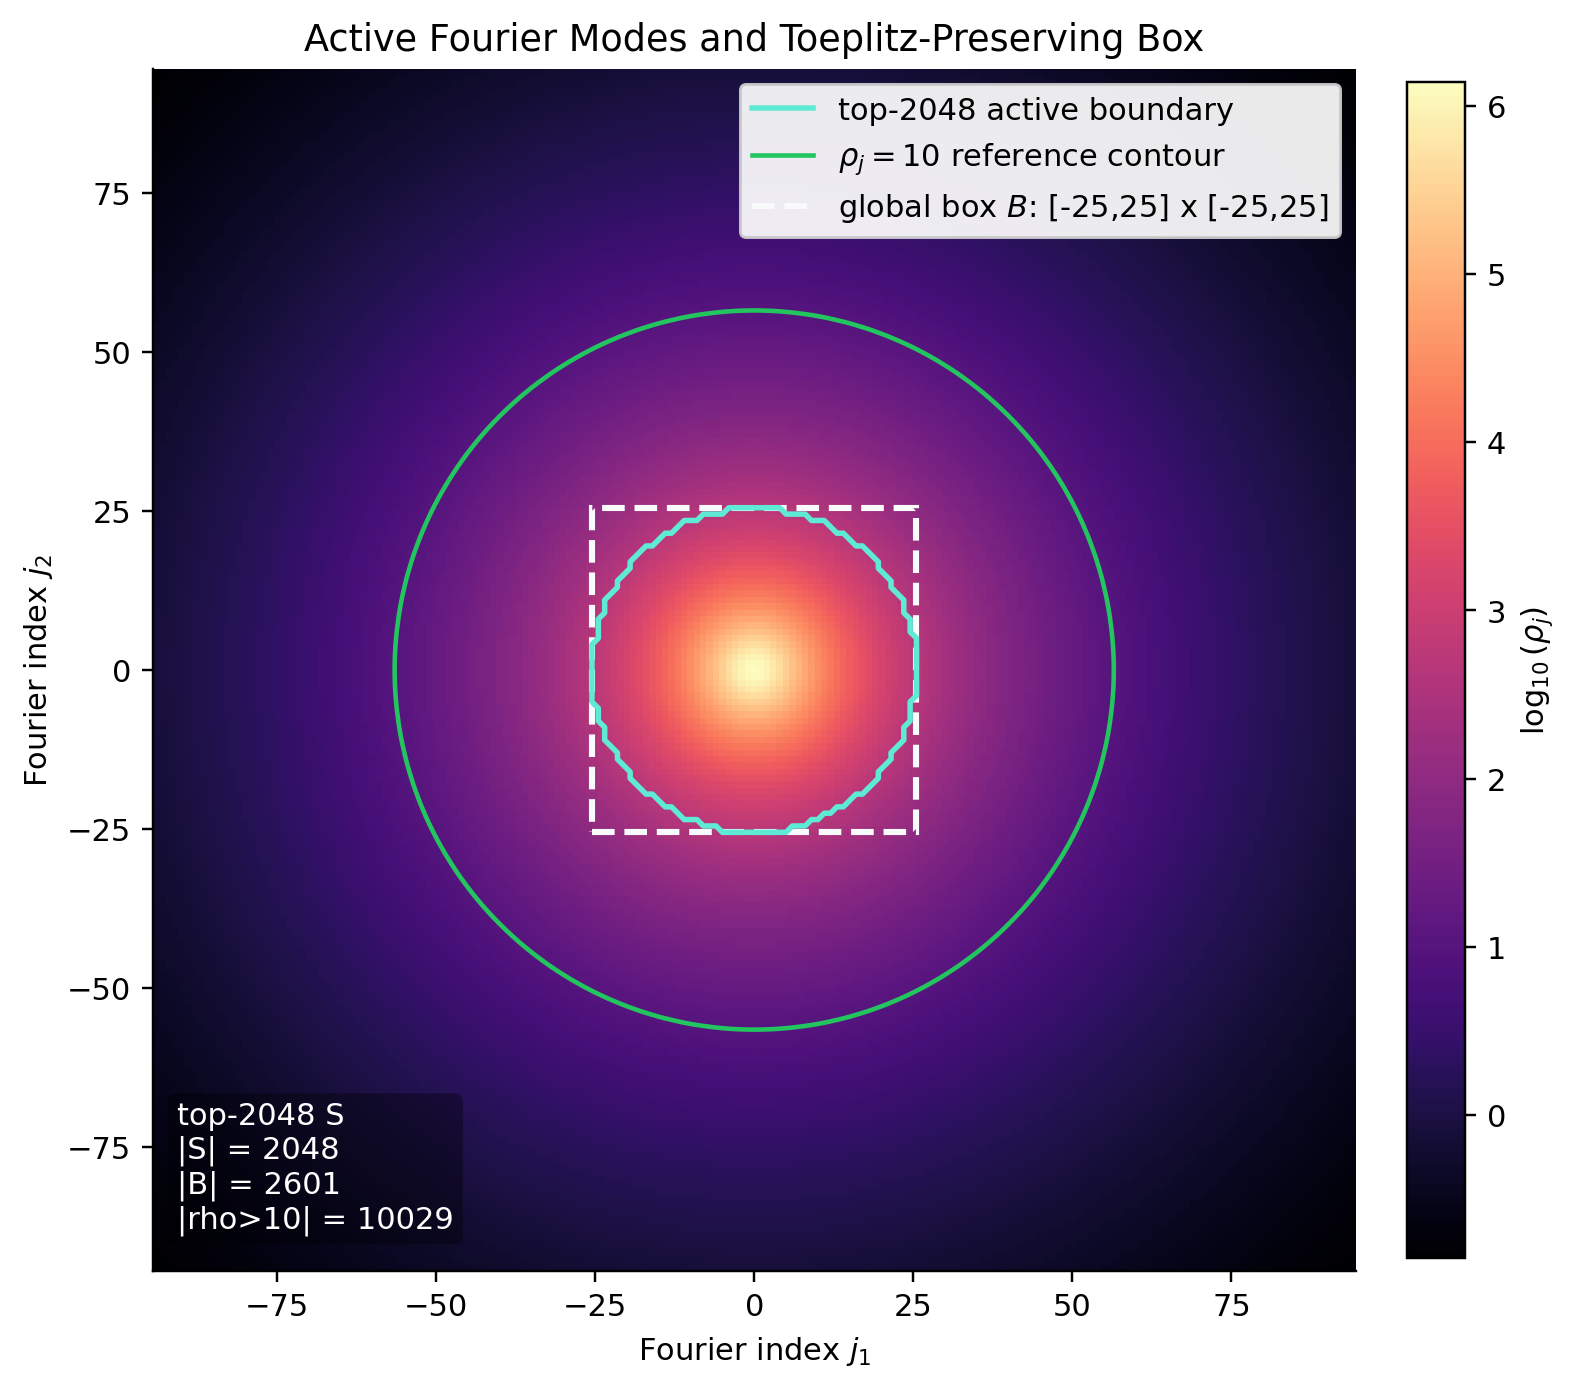
\includegraphics[width=.30\linewidth]{paper_project/picture/active_set_fourier_modes.png}
% \includegraphics[width=.60\linewidth]
% {paper_project/picture/rho_radial_mass_profile.png}
% \caption{ Active Fourier concentration for the KRR problem in \eqref{eq:krr-objective}, solved through the EFGP weight-space system \eqref{eq:weight-space-system} with \(A=DGD+\lambda I_M\) as in \eqref{eq:A-DGD}. For each Fourier mode \(j\in J_m\), we use the signal-to-regularization score \(\rho_j=N|D_{j,j}|^2/\lambda=H_{j,j}/\lambda\) defined in \eqref{eq:rho-score}, and approximate the selected active modes by the smallest Cartesian box \(B\) in \eqref{eq:active-box}. Left: heat map of \(\log_{10}\rho_j\) on the two-dimensional Fourier grid; the top-\(k\) active modes concentrate near the origin, and the dashed square shows the enclosing active box \(B\). The \(\rho_j=10\) contour is shown as a reference regularization scale. Middle: radial profile of \(\rho_j\), showing that the Fourier signal strength decays rapidly as the frequency radius increases; the vertical dashed line marks the active-box radius. Right: cumulative \(\rho\)-mass as a function of radius, showing that the active box captures almost all dominant Fourier spectral mass while retaining a compact Cartesian subgrid. }
% \label{fig:active-fourier-concentration}
% \end{figure}


% Let \(B_\tau\) be the smallest axis-aligned box containing \(S_\tau\). Since \(T_\tau\subseteq J_m\setminus S_\tau\), every \(j\in T_\tau\) satisfies
% \(\rho_j\le \tau\). Therefore
% \begin{equation}
%     H_{j,j}\le \tau\lambda,
%     \qquad j\in T_\tau,
%     \label{eq:tail-diagonal-entry-bound}
% \end{equation}
% and
% \begin{equation}
%     |H_{j,\ell}|
%     \le
%     \lambda\sqrt{\rho_j\rho_\ell}
%     \le
%     \tau\lambda,
%     \qquad j,\ell\in T_\tau .
%     \label{eq:tail-entry-bound}
% \end{equation}
% The entrywise bounds suggest that tail coordinates are individually dominated
% by the regularization scale. They do not by themselves imply spectral diagonal
% dominance of the full tail block; the effectiveness of a diagonal tail
% approximation also depends on the accumulated off-diagonal interactions in
% \(H_{TT}\).These observations motivate the main strategy of this paper: treat the active
% block \(A_{SS}\), or its Toeplitz-preserving box approximation \(A_{BB}\),
% accurately, while applying only a cheap diagonal or approximate correction on
% the complement. The next section makes this idea precise as an active-block
% preconditioner and analyzes the resulting approximation errors.

\subsection{Selecting the active box}
\label{subsec:active-box-selection}

Since \(|F_{n,j}|=1\), \cref{eq:fourier-system} gives
\(G_{j,j}=N\) and \(A_{j,j}-\lambda=N|D_{j,j}|^2\). For distinct
\(j,\ell\in J_m\), it also gives
\[
    A_{j,\ell}
    =
    D_{j,j}D_{\ell,\ell}
    \sum_{n=1}^N
    e^{2\pi i h\langle \ell-j,x_n\rangle},
    \qquad
    |A_{j,\ell}|
    \leq
    N |D_{j,j}|\,|D_{\ell,\ell}|.
\]
Here \(D_{j,j}=\sqrt{h^d\widehat k(hj)}\). We rank the coordinates by
\(\rho_j:=N|D_{j,j}|^2/\lambda=(A_{j,j}-\lambda)/\lambda\). This ratio is the
diagonal contribution of Fourier index \(j\), measured in units of the ridge
term. A large value means that regularization does not dominate that
coordinate, so omitting it from the accurate part of the preconditioner is
risky. A small value also reduces its pairwise interactions with other
small-score coordinates through the preceding bound. The ratio is therefore a
plausible and inexpensive ranking rule, but it does not account for the sum of
many off-diagonal interactions and is not by itself a conditioning guarantee.

For a threshold \(\tau>0\), define
\begin{equation}
    S_\tau
    =\{j\in J_m:\rho_j>\tau\}
    =\{j\in J_m:N|D_{j,j}|^2>\tau\lambda\}.
    \label{eq:threshold-active-set}
\end{equation}
Thus \(\tau=1\) selects coordinates whose unregularized diagonal contribution
exceeds the ridge term. For a selection budget \(s\), let \(S_s\) contain the
\(s\) largest-score indices. These rules have different roles because
\begin{equation}
    \rho_j=\frac{Nh^d}{\lambda}\widehat k(hj).
    \label{eq:score-spectrum-form}
\end{equation}
On a fixed Fourier grid, the ordering used by \(S_s\) is independent of
\(N\) and \(\lambda\), whereas \(S_\tau\) changes with \(N/\lambda\).
The top-\(s\) rule fixes the number of initially selected modes, although the
enclosing box can contain more than \(s\) coordinates; the threshold rule is
regularization-aware. We use \(S_\tau\) as the primary definition and retain
\(S_s\) as a budgeted alternative.

For either rule, write \(S\) for the selected set and enclose it in the
smallest centered Cartesian box
\begin{equation}
    B=\prod_{r=1}^d\{-b_r,\ldots,b_r\},
    \qquad S\subseteq B\subseteq J_m.
    \label{eq:active-cartesian-box}
\end{equation}
We set \(B=\varnothing\) when \(S=\varnothing\). The box can include indices
below the threshold, but it preserves the multilevel Toeplitz structure of
\(G_{BB}\). For a non-full box, define the induced threshold
\begin{equation}
    \tau_B=\max_{j\in J_m\setminus B}\rho_j,
    \label{eq:induced-box-threshold}
\end{equation}
and set \(\tau_B=0\) when \(B=J_m\). The strict inequality in
\cref{eq:threshold-active-set} gives \(B\supseteq S_{\tau_B}\). Consequently,
the Fourier-system bounds in \cref{eq:fourier-system-bounds} also apply to a
box obtained from a top-\(s\) selection. This containment does not assert that
an arbitrary top-\(s\) box obeys the geometric size formula below.

\begin{proposition}[Growth of a threshold box]
\label{prop:threshold-box-growth}
Assume a unit-variance isotropic kernel and let \([u]_+=\max(u,0)\).
The radii below are measured in the integer Fourier index \(j\); the
corresponding frequency radii are \(hR_\tau\).

For the squared exponential kernel
\[
    k_{\mathrm{SE}}(x,z)
    =\exp\!\left(-\frac{\|x-z\|_2^2}{2\ell^2}\right),
\]
define
\begin{equation}
    R_{\mathrm{SE}}(\tau)
    =\frac{1}{\sqrt{2}\pi\ell h}
    \sqrt{\left[
        \log\!\left(
            \frac{Nh^d(\sqrt{2\pi}\ell)^d}{\tau\lambda}
        \right)
    \right]_+}.
    \label{eq:se-active-radius}
\end{equation}
Then
\begin{equation}
    S_\tau
    =J_m\cap\{j\in\mathbb Z^d:\|j\|_2<R_{\mathrm{SE}}(\tau)\}.
    \label{eq:se-active-ball}
\end{equation}

For the unit-variance Mat\'ern parameterization
\[
    k_{\nu,\ell}(x,z)
    =\frac{2^{1-\nu}}{\Gamma(\nu)}
    \left(\frac{\sqrt{2\nu}\|x-z\|_2}{\ell}\right)^\nu
    K_\nu\!\left(\frac{\sqrt{2\nu}\|x-z\|_2}{\ell}\right),
    \qquad \nu>0,
\]
the Fourier convention in \cref{subsec:fourier-expansion} gives
\begin{equation}
    \widehat k_{\nu,\ell}(\xi)
    =c_{\nu,d,\ell}
    \left(2\nu+4\pi^2\ell^2\|\xi\|_2^2\right)^{-\nu-d/2},
    \qquad
    c_{\nu,d,\ell}
    =\frac{2^d\pi^{d/2}(2\nu)^\nu\Gamma(\nu+d/2)}
           {\Gamma(\nu)}\,\ell^d.
    \label{eq:matern-spectrum-active-box}
\end{equation}
These transform formulas use the same \(2\pi\) convention as
\cite[Sec.~4.2]{rasmussen2006gaussian}; see also
\cite{barnett2024uniform}. Define
\begin{equation}
    R_{\mathrm{Mat}}(\tau)
    =\frac{1}{2\pi\ell h}
    \sqrt{\left[
        \left(\frac{Nh^dc_{\nu,d,\ell}}{\tau\lambda}\right)^{2/(2\nu+d)}
        -2\nu
    \right]_+}.
    \label{eq:matern-active-radius}
\end{equation}
Then
\begin{equation}
    S_\tau
    =J_m\cap\{j\in\mathbb Z^d:\|j\|_2<R_{\mathrm{Mat}}(\tau)\}.
    \label{eq:matern-active-ball}
\end{equation}

If \(S_\tau\ne\varnothing\), define
\[
    b_\tau=\max_{j\in S_\tau}\|j\|_\infty.
\]
Its smallest centered box is
\(B_\tau=\{-b_\tau,\ldots,b_\tau\}^d\), and
\begin{equation}
    |B_\tau|=(2b_\tau+1)^d,
    \qquad
    b_\tau\leq
    \min\{m,\lceil R_\tau\rceil-1\},
    \label{eq:threshold-box-cardinality}
\end{equation}
where \(R_\tau\) denotes the applicable radius. If \(R_\tau>m\), then
\(B_\tau=J_m\).
\end{proposition}

With \(d,h,\ell,\tau\) fixed and before truncation by \(J_m\), the exact
radii imply
\begin{equation}
    R_{\mathrm{SE}}(\tau)
    =O\!\left(\sqrt{\log(N/\lambda)}\right),
    \qquad
    |B_{\mathrm{SE}}|
    =O\!\left([\log(N/\lambda)]^{d/2}\right),
    \label{eq:se-box-growth}
\end{equation}
whereas
\begin{equation}
    R_{\mathrm{Mat}}(\tau)
    =O\!\left((N/\lambda)^{1/(2\nu+d)}\right),
    \qquad
    |B_{\mathrm{Mat}}|
    =O\!\left((N/\lambda)^{d/(2\nu+d)}\right).
    \label{eq:matern-box-growth}
\end{equation}
Thus the SE box grows polylogarithmically in \(N/\lambda\), while the
Mat\'ern box grows algebraically. On a finite grid either box can saturate at
\(J_m\); the algebraic Mat\'ern growth can lead to earlier saturation. If the
kernel-approximation tolerance or lengthscale changes \(h\), the exact radii
in \cref{eq:se-active-radius,eq:matern-active-radius} should be used instead
of these fixed-grid growth laws.

%需要进行拆分，考虑只展示重要结果
Let \(B\supseteq S_\tau\) and \(T=J_m\setminus B\). Then
\(\rho_j\leq\tau\) for every \(j\in T\), so
\[
    A_{j,j}-\lambda\leq \tau\lambda,
    \qquad
    |A_{j,\ell}|
    \leq
    \lambda\sqrt{\rho_j\rho_\ell}
    \leq
    \tau\lambda,
    \qquad
    j,\ell\in T,\quad j\ne\ell.
\]

These entrywise bounds do not control their combined operator norm.
\Cref{sec:main-algorithms} therefore analyzes both the approximation on \(T\)
and the coupling between \(B\) and \(T\).


% \paragraph{Toy data example}
% We use a two-dimensional synthetic regression problem to make the structure visible. Figure~\ref{fig:active-fourier-concentration} illustrates the score profile
% on the two-dimensional Mat\'ern synthetic problem used for the mechanism
% diagnostics in Section~\ref{sec:experiments}. The large scores
% are concentrated near low frequencies, and their enclosing Cartesian box
% captures most of the cumulative score mass.

% \begin{figure}[H]
% \centering
% 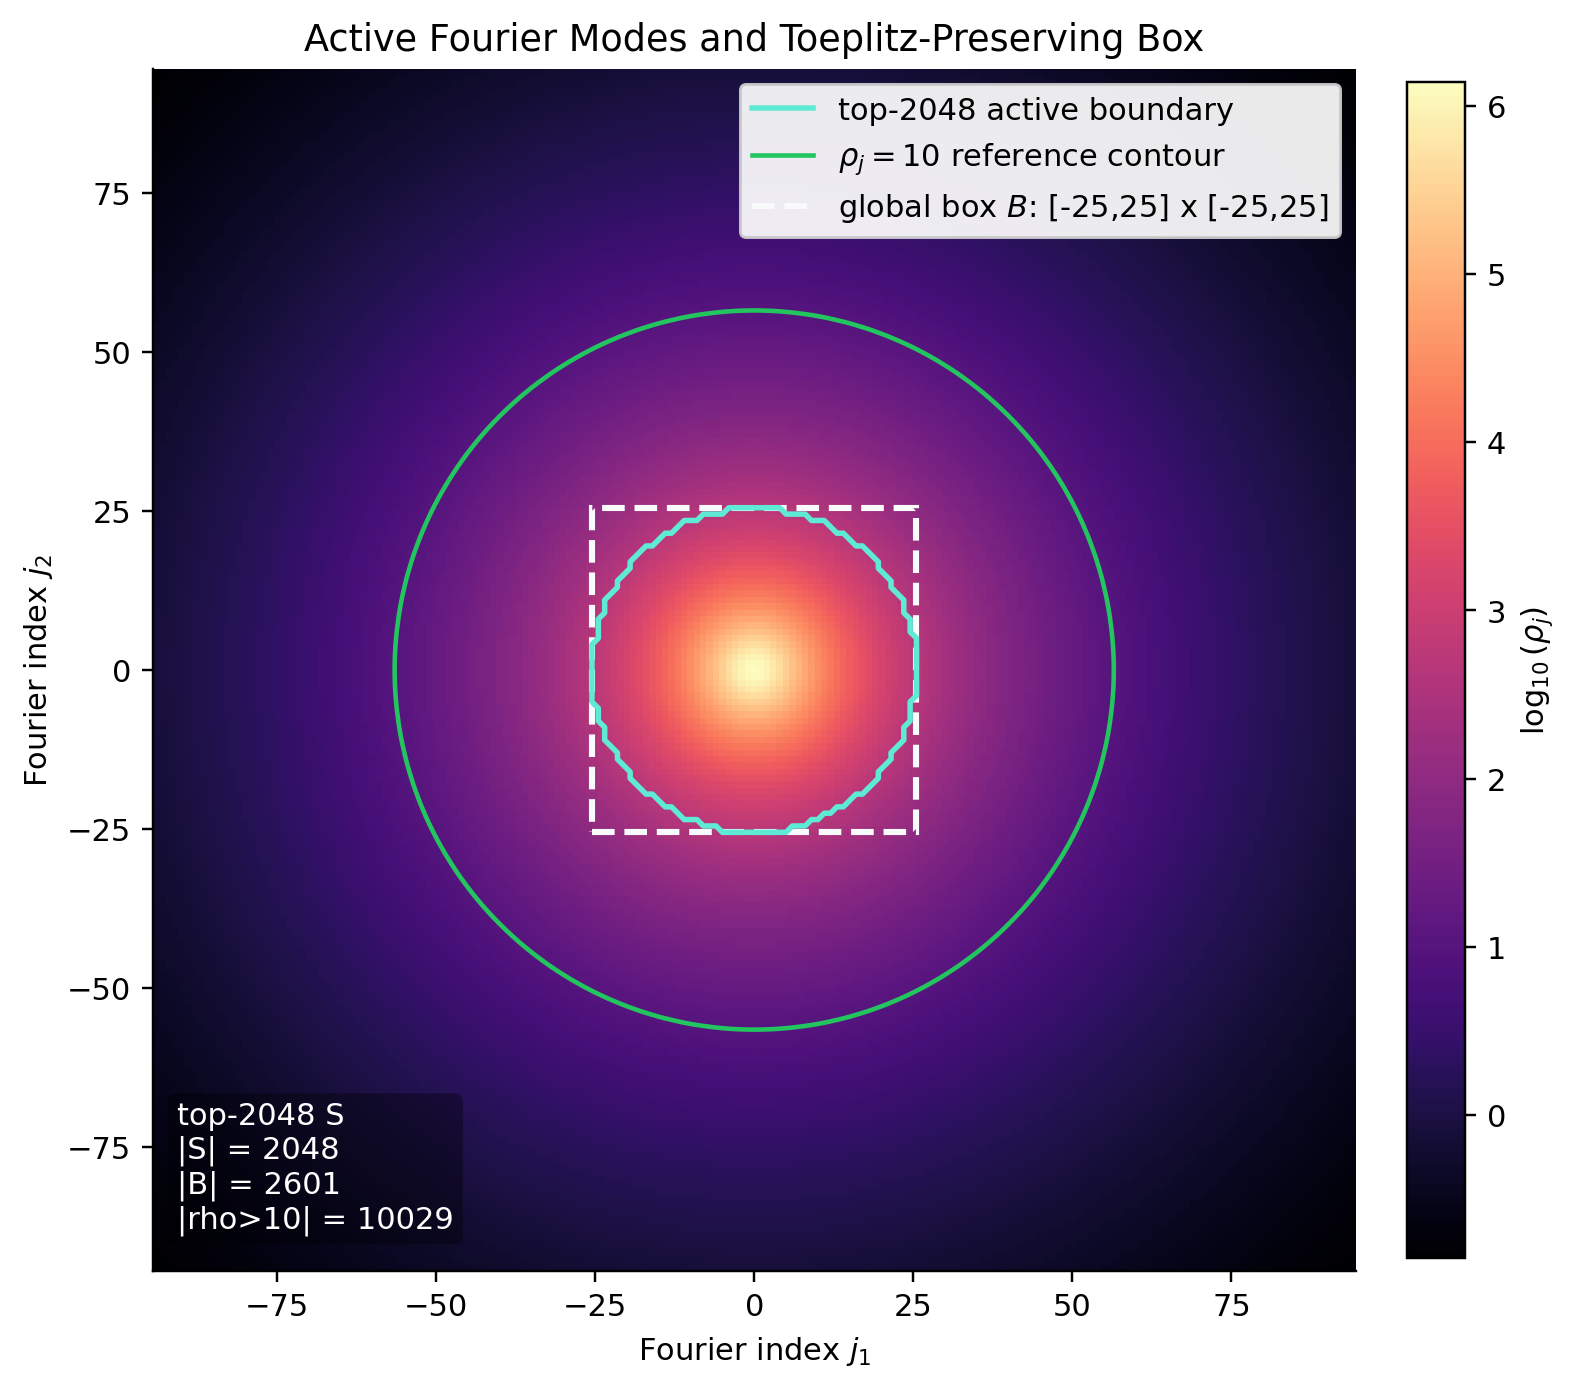
\includegraphics[width=.30\linewidth]{paper_project/picture/active_set_fourier_modes.png}
% \includegraphics[width=.60\linewidth]
% {paper_project/picture/rho_radial_mass_profile.png}
% \caption{ Fourier-score localization on the two-dimensional Mat\'ern synthetic problem. Left: \(\log_{10}\rho_j\) and the selected Cartesian box. Middle: radial score profile. Right: cumulative score mass.
% %Active Fourier concentration for the KRR problem in \eqref{eq:krr-objective}, solved through the EFGP weight-space system \eqref{eq:weight-space-system} with \(A=DGD+\lambda I_M\) as in \eqref{eq:A-DGD}. For each Fourier mode \(j\in J_m\), we use the signal-to-regularization score \(\rho_j=N|D_{j,j}|^2/\lambda=H_{j,j}/\lambda\) defined in \eqref{eq:rho-score}, and approximate the selected active modes by the smallest Cartesian box \(B\) in \eqref{eq:active-box}. Left: heat map of \(\log_{10}\rho_j\) on the two-dimensional Fourier grid; the top-\(k\) active modes concentrate near the origin, and the dashed square shows the enclosing active box \(B\). The \(\rho_j=10\) contour is shown as a reference regularization scale. Middle: radial profile of \(\rho_j\), showing that the Fourier signal strength decays rapidly as the frequency radius increases; the vertical dashed line marks the active-box radius. Right: cumulative \(\rho\)-mass as a function of radius, showing that the active box captures almost all dominant Fourier spectral mass while retaining a compact Cartesian subgrid. 
% }
% \label{fig:active-fourier-concentration}
% \end{figure}
% Let \(B_\tau\) be the smallest axis-aligned box containing \(S_\tau\), and let
% \(T_\tau\subseteq J_m\setminus S_\tau\). Since \(\rho_j\le\tau\) for all
% \(j\in T_\tau\),
% \begin{equation}
%     H_{j,j}\le \tau\lambda,
%     \qquad
%     |H_{j,\ell}|
%     \le \lambda\sqrt{\rho_j\rho_\ell}
%     \le \tau\lambda,
%     \qquad j,\ell\in T_\tau .
%     \label{eq:tail-entry-bounds}
% \end{equation}
% Thus, tail entries are individually controlled by the regularization scale, although this does not by itself guarantee spectral diagonal dominance of \(H_{TT}\). This motivates treating \(A_{SS}\), or its Toeplitz-preserving box approximation \(A_{BB}\), accurately while using only a cheap approximation on the complement.
